\documentclass[oneside,final,14pt,a4paper]{extreport}

\usepackage{iftex}
\ifPDFTeX
  \usepackage{tempora}
  \usepackage[T1,T2A]{fontenc}
  \usepackage[utf8]{inputenc}
  \DeclareFontShape{OT1}{cmtt}{bx}{n}
    {<5><6><7><8><9><10><10.95><12><14.4><17.28><20.74><24.88>cmttb10}{}
  \renewcommand{\ttdefault}{pcr}
\else
  \usepackage{fontspec}
  \setmainfont{Times New Roman}
  \setsansfont{Arial}
  \setmonofont{Courier New}[Scale=MatchLowercase]
\fi

\usepackage[
  a4paper,
  left=25mm,
  right=20mm,
  top=20mm,
  bottom=20mm,
  headheight=17pt,
  headsep=7mm,
  footskip=10mm
]{geometry}

\usepackage{setspace}
\setstretch{1.5}
\setlength{\emergencystretch}{2em}
\usepackage{indentfirst}
\setlength{\parindent}{1.25cm}

\usepackage[english]{babel}

\usepackage{amsmath,amsfonts}
\usepackage{graphicx}
\graphicspath{{figs/}}
\usepackage{booktabs}
\usepackage{longtable}
\usepackage{array}
\usepackage{float}
\usepackage{placeins}
\usepackage{enumitem}
\usepackage{csquotes}
\usepackage{url}
\usepackage{xurl}
\usepackage{xcolor}

\usepackage[
  backend=biber,
  style=ieee,
  autocite=inline
]{biblatex}
\addbibresource{ref.bib}
\DefineBibliographyStrings{english}{bibliography={References}}
\AtBeginBibliography{\sloppy}

\usepackage[
  labelfont=normalfont
]{caption}
\captionsetup[table]{name={Table},labelsep=period,justification=centering,singlelinecheck=false}
\captionsetup[figure]{name={Figure},labelsep=period,justification=raggedright,singlelinecheck=false}

\usepackage{fancyhdr}
\setlength{\headheight}{17pt}
\pagestyle{fancy}
\fancyhf{}
\fancyhead[L]{\nouppercase{\leftmark}}
\fancyhead[R]{\thepage}
\renewcommand{\chaptermark}[1]{\markboth{\chaptername\ \thechapter\ -- #1}{}}

\usepackage[
  colorlinks=true,
  linkcolor=black,
  citecolor=black,
  urlcolor=black
]{hyperref}

\begin{document}

\begingroup
\setstretch{1.0}
\thispagestyle{empty}
\begin{center}
\textbf{Автономная некоммерческая организация высшего образования}\\
\textbf{<<Университет Иннополис>>}

\vspace{0.45cm}

\textbf{\MakeUppercase{Выпускная квалификационная работа}}\\
\textbf{(бакалаврская работа)}\\
\textbf{по направлению подготовки}\\
\textbf{09.03.01 --- <<Информатика и вычислительная техника>>}

\vspace{0.45cm}

\textbf{\MakeUppercase{Graduation Thesis}}\\
\textbf{(Bachelor's Graduation Thesis)}\\
\textbf{Field of Study}\\
\textbf{09.03.01 --- <<Computer Science>>}

\vspace{0.45cm}

\textbf{Направленность (профиль) образовательной программы}\\
\textbf{<<Информатика и вычислительная техника>>}\\
\textbf{Area of Specialization / Academic Program Title:}\\
\textbf{<<Computer Science>>}
\end{center}

\vspace{0.45cm}

\noindent
\begin{tabular}{@{}p{2.7cm}p{12.6cm}@{}}
\textbf{Тема /}\\
\textbf{Topic}
&
\fbox{\begin{minipage}[c][2.6cm][c]{12.2cm}
\textbf{Visual Studio Code Extension for Type-Based Visualization for the Stella Programming Language / Расширение Visual Studio Code для визуализации информации на основе типов для языка программирования Stella}
\end{minipage}}
\end{tabular}

\vspace{0.45cm}

\noindent
\begin{tabular}{@{}p{4.2cm}p{5.5cm}p{4.1cm}@{}}
Работу выполнил /\\
Thesis is executed by
&
\fbox{\begin{minipage}[c][1.9cm][c]{5.1cm}
\textbf{Фадеенков Антон Олегович / Fadeenkov Anton Olegovich}
\end{minipage}}
&
\fbox{\begin{minipage}[c][1.9cm][c]{3.7cm}
\centering \vfill подпись / signature
\end{minipage}}
\\[0.35cm]
Руководитель выпускной квалификационной работы /\\
Supervisor of Graduation Thesis
&
\fbox{\begin{minipage}[c][2.4cm][c]{5.1cm}
\textbf{Кудасов Николай Дмитриевич / Kudasov Nikolay Dmitrievich}
\end{minipage}}
&
\fbox{\begin{minipage}[c][2.4cm][c]{3.7cm}
\centering \vfill подпись / signature
\end{minipage}}
\end{tabular}

\vfill
\begin{center}
Иннополис, Innopolis, 2025
\end{center}
\endgroup
\clearpage

\pagenumbering{arabic}
\setcounter{page}{2}
\tableofcontents
\listoftables
\listoffigures
\chapter*{Abstract}
\addcontentsline{toc}{chapter}{Abstract}

This thesis presents a Visual Studio Code extension for visual analysis of programs written in Stella, an educational statically typed programming language. The problem addressed in this work is that standard editor diagnostics expose the final result of language analysis but do not show the intermediate structures used during parsing and type checking. The developed extension makes five kinds of information available inside the editor: an abstract syntax tree, a scope and typing-context view, a type derivation tree, a reverse type-error trace, and a type dependency graph. The implementation uses TypeScript, the Visual Studio Code Extension API, Langium, and custom Language Server Protocol requests. The client and server are separated so that semantic analysis remains on the language-server side, while editor-specific rendering is implemented on the client side. The prototype was evaluated by the author using six reproducible scenarios for correct and incorrect Stella programs. The evaluation confirmed the availability of the required data, synchronization with source ranges, bidirectional navigation, decomposition of typing steps, and highlighting of type conflicts. These results show that the prototype satisfies the functional criteria used in the evaluation. They do not prove that the extension improves learning outcomes, code readability, or debugging speed for other users because no controlled user study was conducted. A user study with objective task-completion measurements is therefore left for future work.


\clearpage

\chapter{Introduction}
\label{chap:intro}
\chaptermark{Introduction}

\section{Motivation}

Static type systems detect inconsistent operations before program execution and provide information used by compilers and development tools~\cite{Types,HarperPFPL,Gao2017TypeNotType,Hanenberg2010StaticDynamic}. For a student, however, the result of type checking is often visible only as a final type or an error message. The intermediate structures---the abstract syntax tree, the typing context, the applied typing rules, and dependencies between expressions---remain hidden.

This problem is relevant in courses on compilers and programming languages~\cite{DragonBook,Types}. Students are expected to connect source code with formal notation, for example a typing judgment of the form $\Gamma \vdash e : T$. In this notation, $\Gamma$ is the typing context: a finite mapping from identifiers that are available at the current program point to their types. The expression $e$ is assigned type $T$ under this context. When only the final result is shown, it can be difficult to reconstruct which rule was applied and which subexpression caused a mismatch.

Visualization is one way to expose these internal structures. Studies of software, algorithm, and data-structure visualization report that interactive representations can support the formation of mental models and the analysis of abstract processes~\cite{Price1993Taxonomy,Hundhausen2002MetaStudy,Naps2002Engagement,Sorva2013Review,EducationalTechnologyResearch}. Similar motivation is used in tools such as Jeliot and visAST, which connect program text with executable or structural representations for software-language education~\cite{Jeliot3,VisAST}. These studies motivate the interface design in this thesis, but their results cannot be transferred automatically to a new tool or to type-system visualization. The educational effect of the developed extension therefore requires a separate evaluation.

\section{Problem Statement}

Stella is an educational language designed for studying the implementation of static type systems~\cite{Abounegm2024Stella}. Its existing language server performs parsing, name resolution, type checking, and diagnostics. Standard Visual Studio Code features can display syntax highlighting, hover information, and error messages, but they do not provide a built-in representation of Stella typing derivations or semantic dependencies.

The practical problem addressed in this work is the absence of an integrated interface that connects Stella source code with the internal results of semantic analysis. A useful interface should answer the following questions:

\begin{itemize}
    \item Which abstract syntax tree (AST) node corresponds to the current source fragment?
    \item Which variables, parameters, and functions are available at the cursor position?
    \item Which typing rules produce the type of the selected expression?
    \item Which sequence of checks leads to a reported type error?
    \item Which expressions and declarations influence the type of the selected expression?
\end{itemize}

A \emph{type dependency graph} is used in this thesis to answer the last question. It is a directed graph whose nodes represent selected expressions, functions, parameters, local bindings, and related subexpressions. An edge $u \rightarrow v$ means that the type or type-checking result of $v$ depends on information obtained from $u$. For example, in a function application, the argument and the called function have incoming edges to the application node. An edge is marked as conflicting when the connected types violate the relevant typing requirement.

\section{Goal and Research Questions}

The goal of this work is to design and implement a Visual Studio Code extension that exposes Stella syntax and type-analysis information as interactive visual representations linked to source code.

The work addresses two research questions:

\begin{enumerate}[label=\textbf{RQ\arabic*:}, leftmargin=*]
    \item How can the semantic information produced by the Stella language server be represented in Visual Studio Code without mixing different analysis tasks into one overloaded interface?
    \item Does the implemented prototype satisfy the functional criteria of locality, hierarchy, source-code traceability, navigation, and explicit conflict indication in a set of reproducible Stella scenarios?
\end{enumerate}

The research questions deliberately concern the design and functional behavior of the prototype. Claims about improved learning outcomes, perceived usability, code readability, or debugging speed would require a controlled study with representative users and are outside the evidence collected in this work.

\section{Contributions}

The contributions of this work are the following implemented artifacts and evaluation materials:

\begin{enumerate}
    \item A synchronized AST viewer that connects tree nodes with source-code ranges.
    \item A scope and context panel that groups available bindings by the program construct that introduces them.
    \item An interactive type derivation view that represents premises, typing rules, conclusions, and the local context $\Gamma$.
    \item A reverse type-error trace that narrows a diagnostic from an enclosing construct to the conflicting subexpression.
    \item A type dependency graph that shows type-relevant relations between functions, arguments, branches, local bindings, and selected expressions.
    \item A set of custom Language Server Protocol requests and shared data structures used to transfer analysis results from the language server to the extension client.
    \item A set of reproducible validation scenarios and example Stella programs for the implemented views.
\end{enumerate}


\section{Thesis Structure}

Chapter~\ref{chap:background} reviews educational visualization, Stella, and the technologies used by language tools. Chapter~\ref{chap:design} defines the design requirements and evaluation method. Chapter~\ref{chap:implementation} describes the architecture, technology choices, implementation, and evolution of the prototype. Chapter~\ref{chap:evaluation} presents the results before discussing the individual validation scenarios and threats to validity. Chapter~\ref{chap:conclusion} summarizes the answers to the research questions and identifies future work. Appendix~\ref{app:artifacts} lists the implementation artifacts and reproduction steps.




\chapter{Background and Related Work}
\label{chap:background}
\chaptermark{Background and Related Work}

\section{Visualization in Computer Science Education}

Program visualization is used to make structures and execution processes observable and has been classified as a distinct area of software visualization research~\cite{Price1993Taxonomy,Sorva2013Review}. Kogan, Chassidim, and Rabaev evaluated AVDS (Animation and Visualization of Data Structures) in a data-structures course~\cite{EducationalTechnologyResearch}. Their experiment involved 78 students. More than 75\% of the students who used AVDS received grades above 80 points, and the reported mean System Usability Scale score was 79.17.

The System Usability Scale (SUS) is a ten-item questionnaire used to obtain a single perceived-usability score in the range from 0 to 100~\cite{Brooke1996SUS,Bangor2009SUS,ISO924111}. The result is an index, not a percentage of correctly completed tasks. Therefore, the value 79.17 describes participants' subjective assessment of AVDS usability; it does not directly measure learning or prove the usability of another visualization tool.

Aalvik's visAST project applies visualization to abstract syntax trees~\cite{VisAST}. Its main purpose is to help students connect source text, grammar concepts, and the hierarchical AST representation. The project is particularly relevant to this thesis because it treats source-to-structure navigation as part of the learning interface. At the same time, visAST focuses on syntax, while this work also visualizes scope, typing derivations, errors, and dependencies.

The related studies support the general motivation for visualization and program comprehension support~\cite{Sorva2013NotionalMachines,Storey2005ProgramComprehension}, but they do not provide empirical evidence for the particular Stella extension developed in this work. For this reason, their findings are used as design background rather than as proof of the effectiveness of the prototype.

\section{Stella and Static Type Systems}

Stella (Statically Typed Extensible Language for Learning Advanced Compiler Construction) is designed for teaching the implementation of type systems~\cite{Abounegm2024Stella,StellaLanguageDocumentation}. The language supports a core calculus and extensions that introduce additional type-system features. This structure allows course assignments to progress from basic typing rules to more advanced language constructs.

A type checker can be described using judgments such as
\[
    \Gamma \vdash e : T,
\]
where $\Gamma$ denotes the typing context, $e$ is an expression, and $T$ is its type~\cite{Types,HarperPFPL,NielsonProgramAnalysis}. The context records assumptions available at the current point, for example $x:\texttt{Nat}$. A derivation tree explains a judgment by showing the premises required by a typing rule and the conclusion produced by that rule.

An AST, a typing context, and a derivation tree answer different questions. The AST describes syntactic composition. The context describes available identifiers and their types. The derivation tree explains why an expression has a type. A type dependency graph provides another view: it emphasizes relations between type-relevant program elements instead of reproducing the complete proof structure. Keeping these models separate is an important design decision of this work.

\section{Language Server Protocol}

The Language Server Protocol (LSP) standardizes communication between an editor client and a language server and uses JSON-RPC as the underlying message format~\cite{MicrosoftLSP,JSONRPC20}. The protocol defines common operations such as diagnostics, completion, hover information, and navigation to definitions. This separation allows language analysis to remain independent from a particular editor.

The standard LSP methods do not define responses for Stella-specific derivation trees, scope frames, or type dependency graphs. However, LSP permits custom requests. The implementation in this work uses this extension point: the server produces semantic data, shared TypeScript interfaces define the response format, and the Visual Studio Code client renders the result. This preserves the client--server boundary while supporting domain-specific visualizations.

After this definition, the shortened form \emph{LSP} is used consistently.

\section{Visual Studio Code Extension API}

The Visual Studio Code Extension API provides commands, editor events, tree views, decorations, and webviews~\cite{MicrosoftVS,VSCodeTreeView,VSCodeWebview}. Tree views are suitable for structures that naturally use parent--child navigation, such as an AST or nested scope frames. Webviews provide more control over layout and interaction and are therefore suitable for proof-like derivation trees, error traces, and dependency graphs.

The API also provides source positions and ranges. These ranges are essential for the design in this thesis because every meaningful visual node can be connected to the corresponding fragment of Stella code. The same mechanism supports both directions of navigation: an editor selection updates a view, and a click in a view reveals the source fragment.

\section{Research Gap}

Existing work provides evidence that visualization can be useful in computer science education and demonstrates tools for algorithm, program, and AST visualization~\cite{Hundhausen2002MetaStudy,Naps2002Engagement,EducationalTechnologyResearch,Jeliot3,VisAST}. Stella provides a structured environment for learning type-system implementation~\cite{Abounegm2024Stella}. LSP and the Visual Studio Code Extension API provide the technical basis for integrating language analysis with an editor~\cite{MicrosoftLSP,MicrosoftVS}.

The remaining gap is a Stella-specific interface that exposes several stages of type analysis and keeps them connected to source code. The gap is practical rather than theoretical: this work does not introduce a new typing algorithm. It transforms existing syntax and type information into coordinated views for program inspection. The next chapter defines the requirements used to design and evaluate these views.



\chapter{Design and Methodology}
\label{chap:design}
\chaptermark{Design and Methodology}

\section{Design Objective}

The extension is designed as an explanatory layer over the existing Stella language services. It does not replace parsing or type checking. Instead, it requests analysis results from the language server and presents them in a form connected to the editor. This boundary is important because a visualization must not introduce a second, inconsistent implementation of the Stella type system.

The design starts from user questions rather than from available UI components. When reading code, a user may need to understand its syntactic structure, the names visible at a position, the derivation of a type, the source of a diagnostic, or the data that influences a type-checking result. These tasks use related information but require different representations.

\section{Design Requirements}

Five functional requirements were defined before evaluating the prototype.

\begin{table}[htbp]
\centering
\caption{Design requirements for the visual analysis extension}
\label{tab:design-requirements}
\begin{tabular}{p{1.2cm}p{4.0cm}p{8.0cm}}
\toprule
\textbf{ID} & \textbf{Requirement} & \textbf{Observable condition} \\
\midrule
R1 & Locality & A view is built for the active source position or selected expression and avoids unrelated program data. \\
R2 & Hierarchical explanation & A compound expression is decomposed into smaller AST nodes, typing premises, or diagnostic steps. \\
R3 & Source traceability & Every meaningful visual element contains a source range when such a range exists. \\
R4 & Bidirectional navigation & Editor selection updates a view, and selecting a visual element reveals the corresponding source fragment. \\
R5 & Explicit conflict indication & Type mismatches are distinguished from valid dependencies and ordinary nodes. \\
\bottomrule
\end{tabular}
\end{table}

The requirements are intentionally observable. Terms such as \enquote{easy to understand} or \enquote{readable} depend on a user's experience and should be measured in a user study or interpreted through established usability and visualization principles~\cite{GreenPetre1996,WareInfoVis}. In contrast, it is possible to verify whether a graph contains a conflict edge or whether a click reveals the expected source range.

\section{Separation of Visual Representations}

The prototype uses five coordinated views.

\subsection{Abstract Syntax Tree}

The AST view represents the hierarchical composition of the program. It is suitable for answering which language construct contains the cursor and how a compound expression is divided into child nodes. A native tree interface supports expansion and collapse and preserves a familiar editor interaction.

\subsection{Scope and Typing Context}

Scope and typing context are closely related but not identical concepts. Scope determines which declarations are visible at a program position. The typing context $\Gamma$ associates the visible names with their types. In the interface, this information is represented as nested frames. A frame identifies the construct that introduced bindings, such as the program, a function, a lambda abstraction, a \texttt{let} expression, or a pattern.

For example, in
\begin{verbatim}
fn(x: Nat) => let y = succ(x) in y
\end{verbatim}
the context at the final occurrence of \texttt{y} contains the function parameter $x:\texttt{Nat}$ and the local binding $y:\texttt{Nat}$. Showing the bindings in separate frames preserves their origin instead of flattening them into one list.

\subsection{Type Derivation Tree}

A type derivation tree represents a judgment as a conclusion supported by zero or more premises. For the expression \texttt{succ(x)}, where $x:\texttt{Nat}$ is available, a simplified derivation is
\[
\frac{\Gamma \vdash x : \texttt{Nat}}
     {\Gamma \vdash \texttt{succ}(x) : \texttt{Nat}}
\;\textsc{T-Succ}.
\]
The view therefore needs a proof-oriented layout rather than a conventional vertical list. Each node stores the rule name, conclusion, premises, expression text, inferred type, relevant part of $\Gamma$, and source range.

Only bindings relevant to the current expression should be displayed when possible. Repeating the complete program context at every node creates long judgments and hides the rule being explained. This is a design choice for locality, not a change to the formal typing relation.

\subsection{Reverse Type-Error Trace}

The error-trace view starts from a diagnostic and follows a narrowing sequence toward the conflicting expression. For
\begin{verbatim}
if true then 0 else false
\end{verbatim}
the trace should show the conditional-expression check, the requirement that both branches have compatible types, and the observed branch types \texttt{Nat} and \texttt{Bool}. Syntax diagnostics are excluded because parser-token expectations do not form a type derivation and would produce misleading output.

A chain is used instead of a complete derivation tree. The purpose is to retain the diagnostic path that is relevant to the current mismatch rather than show every valid part of the expression.

\subsection{Type Dependency Graph}

The type dependency graph is a directed graph $G=(V,E)$. The idea is related to program dependence graphs and slicing, but the graph in this work is local and type-oriented rather than a complete program-dependence representation~\cite{Ferrante1987PDG,Weiser1981Slicing,Horwitz1990Slicing}. The set $V$ contains type-relevant program entities: functions, parameters, local bindings, cases, expressions, and the selected node. An edge $(u,v)\in E$ states that checking the type of $v$ uses information associated with $u$. Edges may have labels such as \texttt{argument}, \texttt{condition}, \texttt{then}, \texttt{else}, \texttt{value}, or \texttt{return}.

For the application \texttt{takesNat(flag)}, the function declaration and the argument are dependencies of the application. If \texttt{takesNat} expects \texttt{Nat} but \texttt{flag} has type \texttt{Bool}, the argument edge and the related node are marked as conflicts. The graph does not claim to be a complete program-dependence graph. It is a local explanatory graph constructed for the selected expression and its type-checking relations.

\section{Connection to Source Code}

A shared range representation is used across all custom responses. A range contains start and end positions in a source document. The client converts this representation to a Visual Studio Code range and uses it for highlighting and navigation.

This design establishes a common interaction rule. Moving the cursor selects the deepest relevant AST node and refreshes position-dependent views. In the opposite direction, clicking an AST item, scope binding, derivation step, trace step, or dependency-graph node reveals its range in the editor. The views therefore remain secondary representations of the same source document rather than independent diagrams.

\section{Client--Server Boundary}

The language server owns parsing, AST traversal, scope computation, type inference, and construction of semantic relations. The extension client owns command registration, editor event handling, view state, layout, and source highlighting. Shared TypeScript interfaces define the protocol boundary.

This separation follows the general LSP architecture~\cite{MicrosoftLSP}. It also reduces the risk of semantic disagreement: the client renders types returned by the server instead of implementing type rules again. Custom requests are used because the standard protocol has no messages for the five Stella-specific representations.

\section{Evaluation Methodology}

The prototype is evaluated through scenario-based functional validation, following the general principle that software-engineering evaluations should make their procedure, context, and validity limitations explicit~\cite{Wohlin2012Experimentation,RunesonHost2009}. Each scenario defines an input program, a cursor position or selected expression, an action, and an observable expected result. The scenarios cover both correct programs and programs with type mismatches.

The method answers RQ2 by checking the requirements in Table~\ref{tab:design-requirements}. It can confirm, for example, that selecting a derivation node reveals a source range and that incompatible conditional branches are marked in a graph. It cannot determine whether a representative student completes a task faster, makes fewer mistakes, or reports a better usability score.

The author executed the scenarios manually in the extension development environment and compared the observed state with the expected result. Example programs and expected graph behavior are included with the artifact and listed in Appendix~\ref{app:artifacts}. The evaluation results and limitations are reported in Chapter~\ref{chap:evaluation}.


\chapter{Implementation}
\label{chap:implementation}
\chaptermark{Implementation}

\section{Architecture}

The implementation consists of three layers. The first layer is the Stella language server. It parses a document, resolves names, performs type analysis, and handles custom requests. The second layer contains shared protocol and analysis types. These interfaces describe AST nodes, scope frames, derivation nodes, trace steps, dependency nodes, edges, and source ranges. The third layer is the Visual Studio Code extension client, which requests data and renders tree views or webviews.

The extension registers commands for showing the derivation tree, error trace, dependency graph, and AST in JSON form. It also creates persistent AST and scope views in the Stella activity-bar container. Editor-selection events are used to keep position-dependent information synchronized with the active document.

\section{Technology Stack and Rationale}

Table~\ref{tab:technology-stack} summarizes the selected technologies and their relation to the design requirements.

\begin{table}[htbp]
\centering
\caption{Technology stack and design rationale}
\label{tab:technology-stack}
\begin{tabular}{>{\raggedright\arraybackslash}p{3.8cm}>{\raggedright\arraybackslash}p{4.1cm}>{\raggedright\arraybackslash}p{7.1cm}}
\toprule
\textbf{Technology} & \textbf{Role} & \textbf{Reason for selection} \\
\midrule
TypeScript & Client, server, and shared protocol types & One type system across the boundary makes request and response structures explicit and reduces accidental disagreement between layers~\cite{TypeScriptHandbook}. \\
Langium & Stella grammar, AST, documents, and language services & The existing Stella server already uses Langium, so the visual analysis can reuse parsed documents and language-service infrastructure instead of introducing another parser~\cite{LangiumDocs}. \\
LSP client library & Communication between the editor and server & The protocol preserves separation between semantic computation and presentation and supports custom Stella requests~\cite{MicrosoftLSP,JSONRPC20}. \\
Visual Studio Code Extension API & Commands, events, tree views, decorations, and panels & The target users work in Visual Studio Code, and the API provides direct access to source ranges and native editor interaction~\cite{MicrosoftVS,VSCodeTreeView,VSCodeWebview}. \\
HTML, CSS, and JavaScript in webviews & Derivation, trace, and graph layout & These views need proof rules, cards, directed edges, and click handling that cannot be expressed clearly with a standard tree view. \\
\bottomrule
\end{tabular}
\end{table}

The Stella services also use Typir as type-system infrastructure on top of Langium~\cite{Typir}. The stack is therefore aligned with the design. TypeScript and shared interfaces support a stable client--server contract. LSP enforces architectural separation. Native tree views are used for hierarchical navigation, while webviews are limited to representations that require custom layout. Source ranges are retained in every layer to satisfy traceability and navigation requirements.

\section{Custom LSP Requests}

The implementation introduces the following custom methods:

\begin{itemize}
    \item \texttt{stella/syntaxTree} returns the document AST in a serializable form;
    \item \texttt{stella/scope} returns the active node and nested scope frames;
    \item \texttt{stella/typeDerivation} returns a recursive proof-like derivation;
    \item \texttt{stella/typeErrorTrace} returns a diagnostic and an ordered trace;
    \item \texttt{stella/typeDependencyGraph} returns graph nodes, edges, labels, types, and conflict markers.
\end{itemize}

Each request contains a document URI and, where required, a cursor position. The server resolves the current Langium document and selects the smallest relevant AST node. A null response is allowed when the cursor does not correspond to a visualizable construct. This behavior lets the client show a clear placeholder instead of failing.

\section{AST Visualization}

The AST is rendered with the Visual Studio Code tree-view API. Each serialized node contains an identifier, a label, child nodes, and a source range. The synchronization controller searches for the deepest node that contains the cursor position. Selecting an item performs the reverse operation and reveals the stored range.

Figure~\ref{fig:ast} shows the AST panel next to the corresponding Stella source. The highlighted \texttt{Abstraction} node and highlighted source region demonstrate the source-to-tree connection. The hover text also displays the selected AST node type and a compact subtree.

\begin{figure}[htbp]
    \centering
    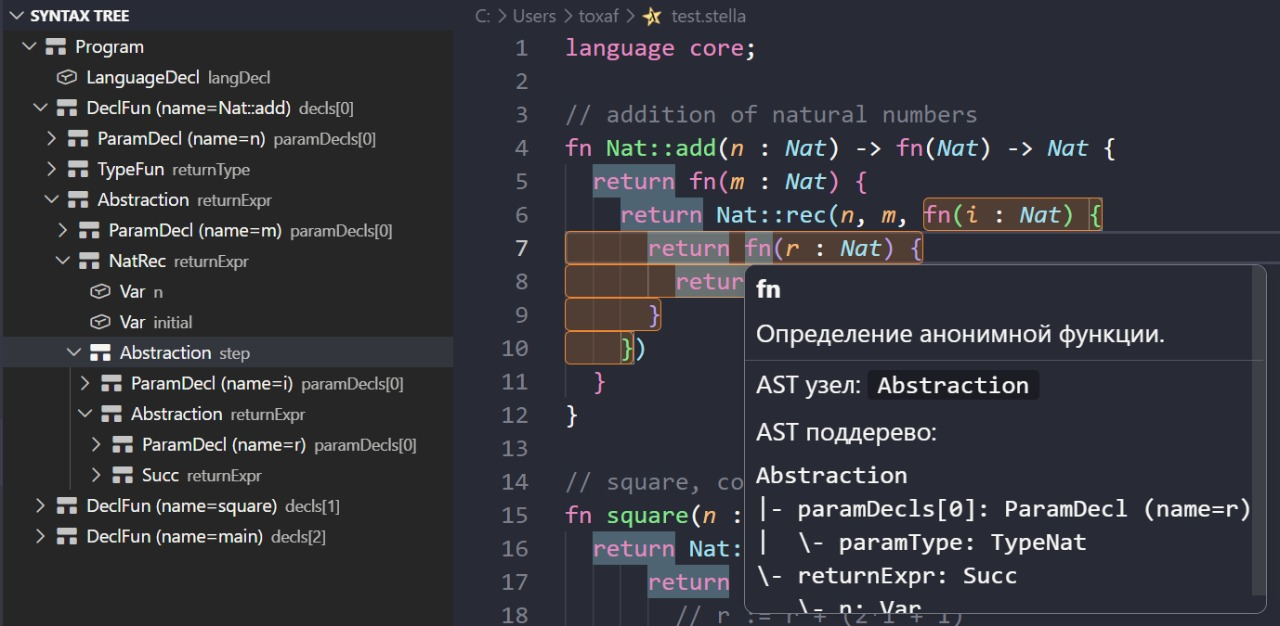
\includegraphics[width=\textwidth]{figs/ast.jpg}
    \caption[Synchronized AST view for a Stella function]{Synchronized AST view for a Stella function. The selected \texttt{Abstraction} node in the tree corresponds to the highlighted nested function in the editor; the hover panel shows the node kind and a textual subtree.}
    \label{fig:ast}
\end{figure}

\section{Scope and Context View}

The server constructs scope frames from ancestors of the active AST node. Separate handlers collect program declarations, function parameters, local declarations, \texttt{let} bindings, recursive bindings, and variables introduced by patterns. Type labels are obtained from explicit annotations or inferred type information when available.

The client renders each frame as a collapsible group and each binding as a child item. Figure~\ref{fig:context} shows three frames: a lambda frame, a function frame, and the program frame. This presentation makes it possible to distinguish the local parameter \texttt{m}, the outer function parameter \texttt{n}, and globally declared functions.

\begin{figure}[htbp]
    \centering
    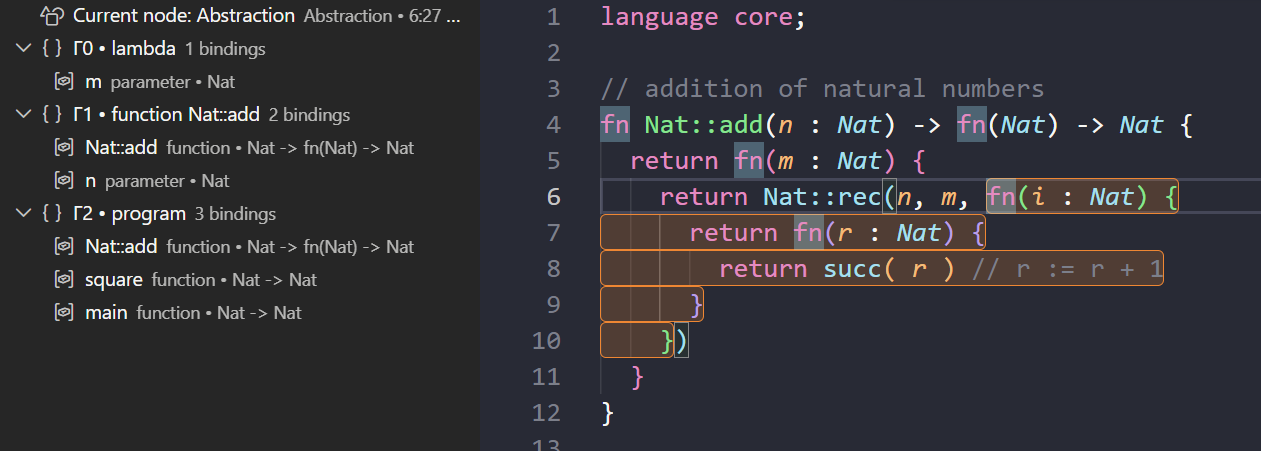
\includegraphics[width=\textwidth]{figs/context_panel.png}
    \caption[Scope and typing-context view for a nested abstraction]{Scope and typing-context view at a nested Stella abstraction. Frames $\Gamma_0$, $\Gamma_1$, and $\Gamma_2$ separate bindings introduced by the lambda, the enclosing function, and the program; each binding includes its role and type.}
    \label{fig:context}
\end{figure}

\section{Type Derivation View}

The server builds a recursive \texttt{TypeDerivationNode}. A node contains a rule name, a conclusion, zero or more premises, a source range, expression text, inferred type, and context text. The client renders premises above a horizontal rule and the conclusion below it.

Figure~\ref{fig:derivation} shows a derivation for nested abstractions ending in \texttt{succ(r)}. The path includes \textsc{T-Var}, \textsc{T-Succ}, and two \textsc{T-Abs} applications. A click on any rule sends its range back to the extension and highlights the corresponding source fragment.

\begin{figure}[htbp]
    \centering
    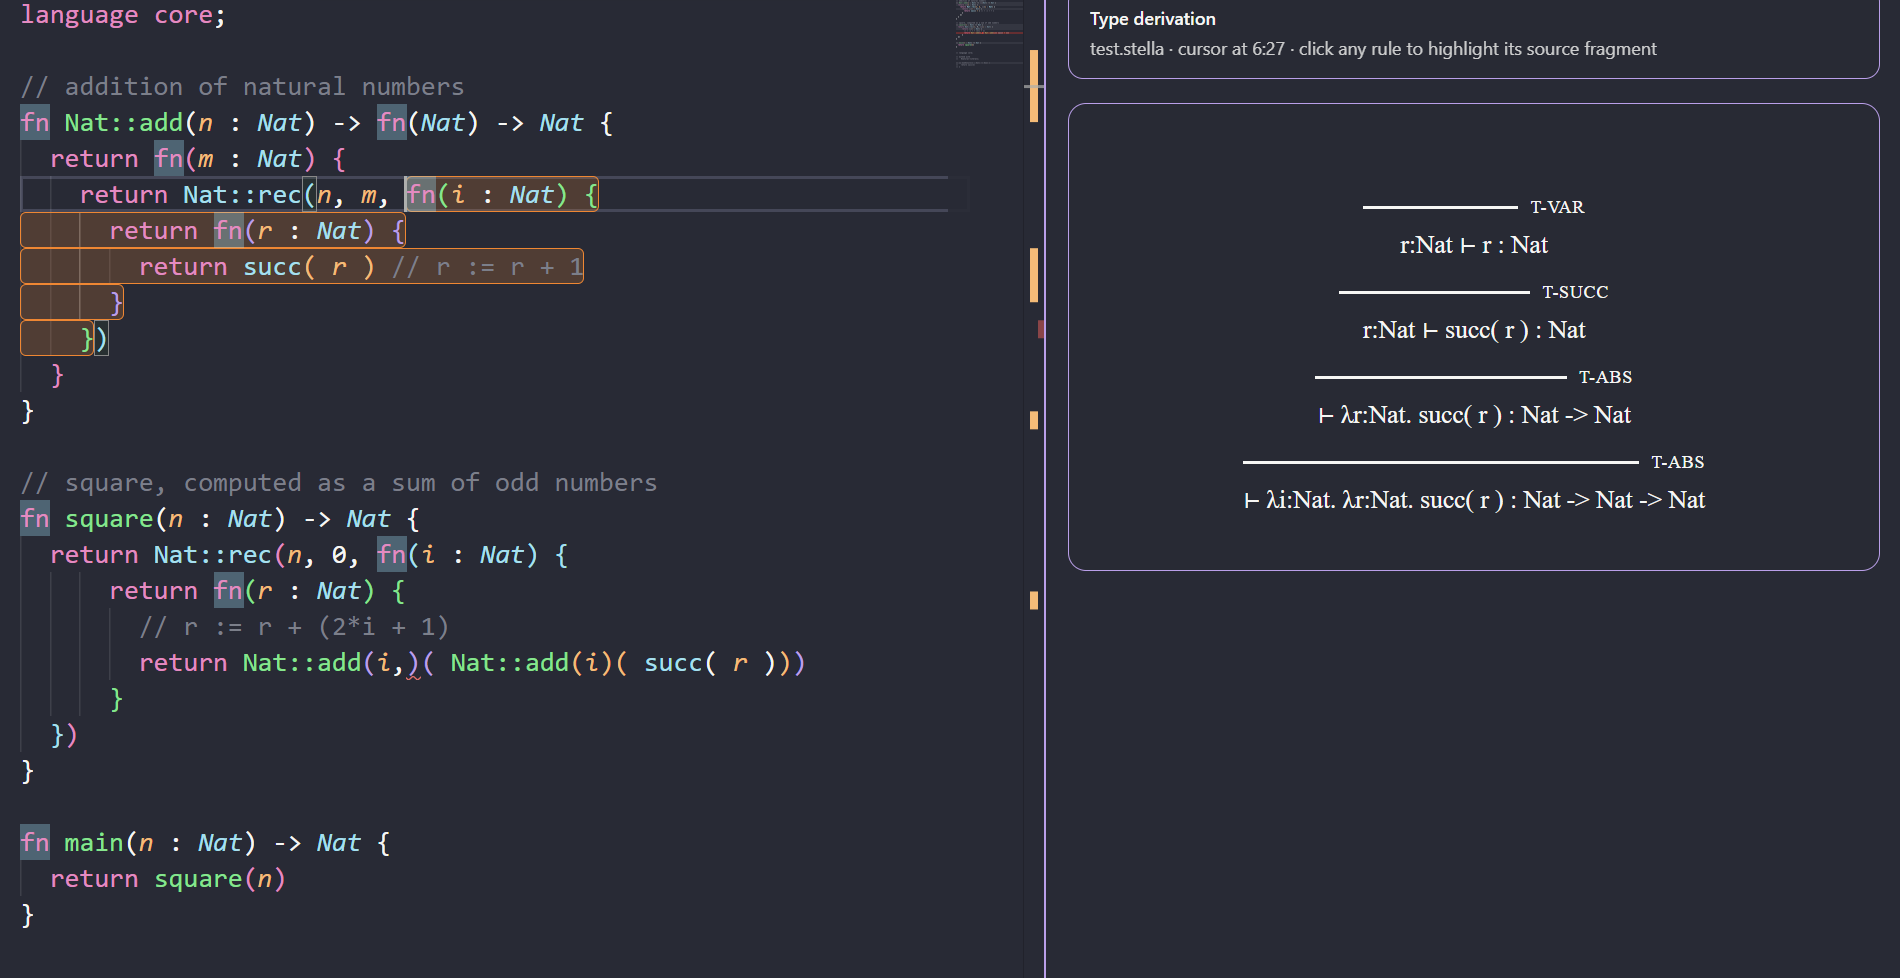
\includegraphics[width=\textwidth]{figs/derivation_tree.png}
    \caption[Interactive type derivation for nested abstractions]{Interactive type derivation for nested Stella abstractions. Premises are placed above rule lines, conclusions below them, and the editor highlights the source fragment associated with the selected derivation step.}
    \label{fig:derivation}
\end{figure}

\section{Type-Error Trace}

The error-trace command first chooses a type-related diagnostic near the cursor. Parser diagnostics and token-expectation messages are filtered out. The server then builds a sequence of related expressions and checks. Each step contains a rule name, judgment, explanation, type information, and source range.

Figure~\ref{fig:error-trace} shows a function declared to return \texttt{Bool} whose body \texttt{succ(n)} has type \texttt{Nat}. The first card states the function contract, and the next card identifies the computed body type. The red border distinguishes the conflict path from an ordinary derivation.

\begin{figure}[htbp]
    \centering
    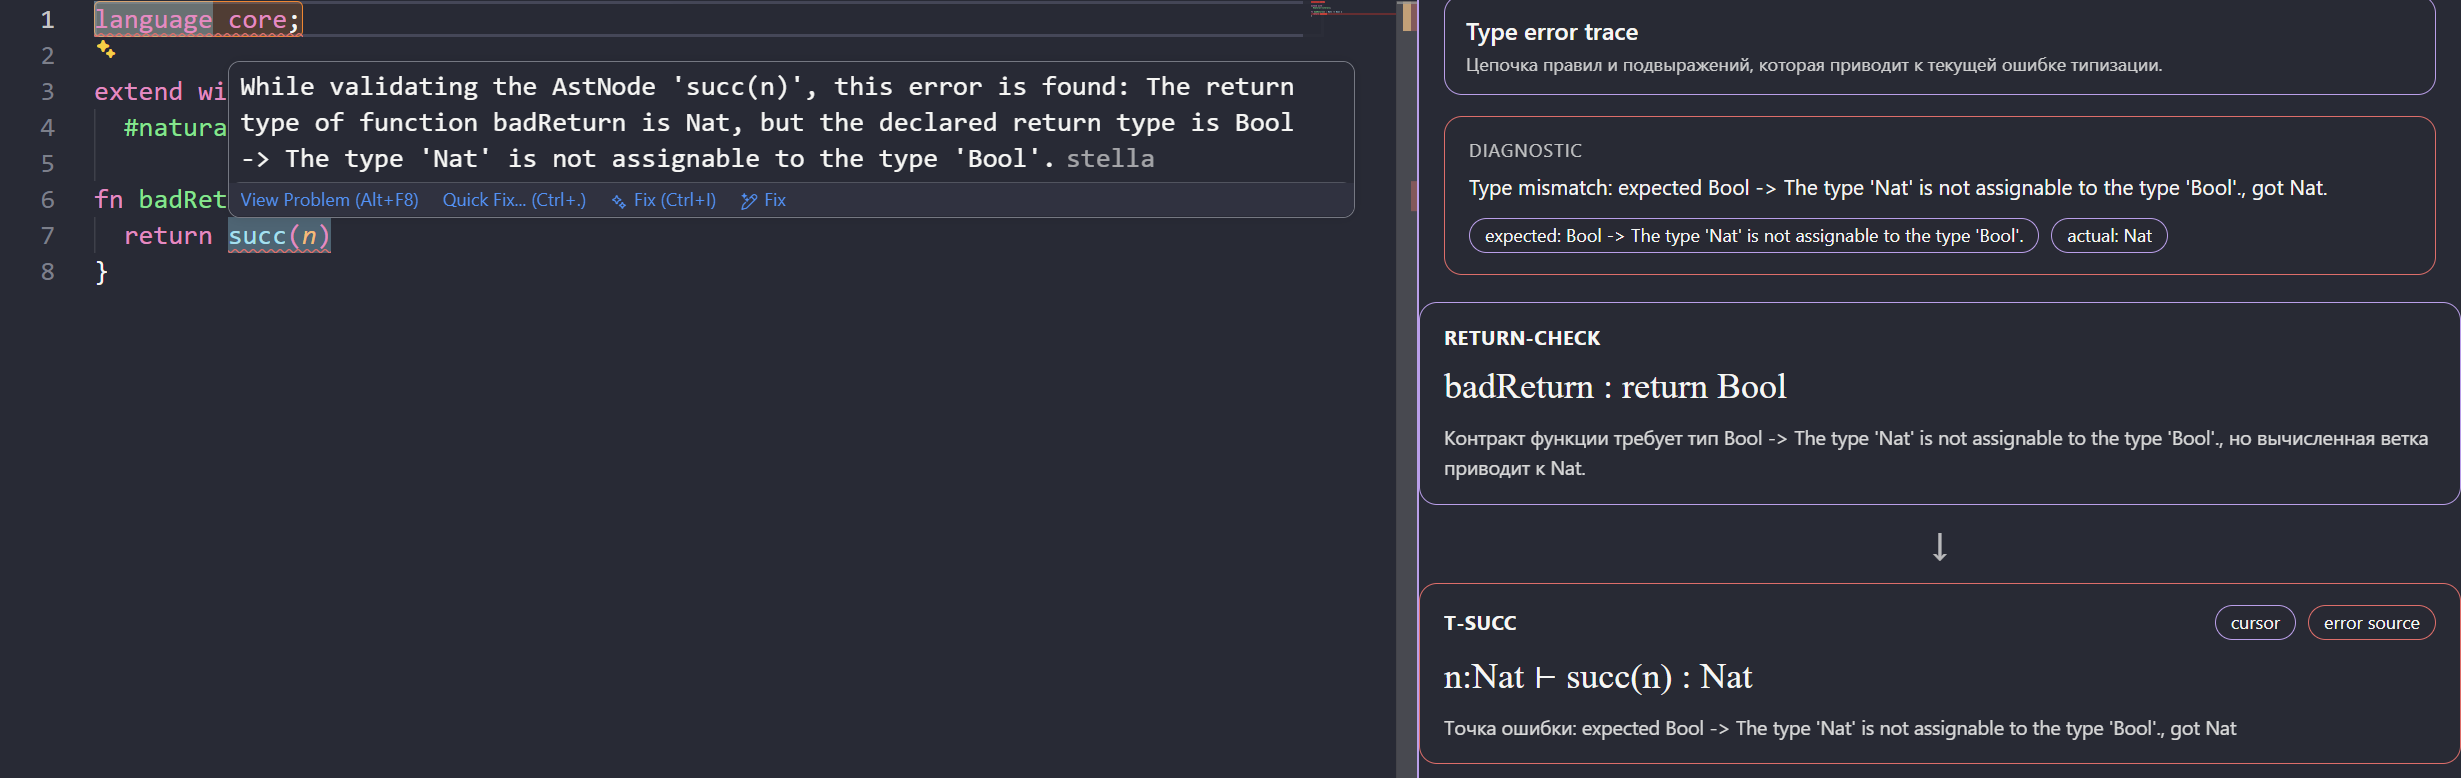
\includegraphics[width=\textwidth]{figs/error_trace.png}
    \caption[Reverse trace for a return-type mismatch]{Reverse trace for a return-type mismatch. The trace connects the declared \texttt{Bool} result of \texttt{badReturn} with the \textsc{T-Succ} judgment that gives \texttt{succ(n)} type \texttt{Nat}; the conflicting source expression is highlighted.}
    \label{fig:error-trace}
\end{figure}

\section{Type Dependency Graph}

The dependency-graph server handler creates nodes for the selected expression and relevant functions, parameters, bindings, cases, and child expressions. Nodes are assigned layers so that dependencies are displayed from left to right. Directed edges are labeled according to their role in type checking.

For a function application, the graph connects the called function and each argument to the application. For a conditional expression, it creates edges for the condition, the \texttt{then} branch, and the \texttt{else} branch. For a \texttt{let} expression, the value flows into its binding, and references to that binding flow into later expressions. The enclosing function is connected through a \texttt{return} relation.

Figure~\ref{fig:dependency-graph} illustrates the graph structure on a simplified argument-mismatch example. The actual webview uses the same logical model, but renders the nodes as clickable elements and applies visual conflict styling to the marked relation.

\begin{figure}[htbp]
    \centering
    \[
    \begin{array}{ccc}
        \texttt{takesNat : Nat -> Nat} & \xrightarrow{\texttt{callee}} & \texttt{takesNat(flag)} \\[0.8em]
        \texttt{flag : Bool} & \xrightarrow{\texttt{argument/conflict}} & \texttt{takesNat(flag)}
    \end{array}
    \]
    \caption[Type dependency graph for an argument mismatch]{Simplified type dependency graph for an argument mismatch. The application depends on the called function and on the argument expression; the argument edge is marked as conflicting because \texttt{flag} has type \texttt{Bool}, while \texttt{takesNat} expects \texttt{Nat}.}
    \label{fig:dependency-graph}
\end{figure}

The server compares available type labels with rule expectations. A mismatching argument or incompatible pair of branches sets \texttt{isConflict} on the corresponding nodes and edges. The webview uses the Visual Studio Code error color for these elements. Clicking a graph node reveals its source range, so the graph remains connected to the selected program.

\section{Evolution of the Prototype}

The implementation was developed in several iterations.

The first iteration exposed the AST and synchronized it with the cursor. This established stable node identifiers and source ranges. The second iteration added scope information. An initial flat list of names was replaced with nested frames after it became clear that a flat list did not explain where a binding originated.

The third iteration introduced the type derivation tree. The first version repeated a large context in each judgment and sometimes stopped decomposition at expressions that were still too complex. The displayed context was then reduced to bindings relevant to a subexpression, and additional expression cases were decomposed into premises. This change reduced repeated context and increased the number of displayed derivation steps, although its effect on human task performance was not measured.

The fourth iteration added reverse error tracing. Early output included parser diagnostics, which produced long token-expectation messages unrelated to typing. Diagnostic filtering and shorter explanations were added to keep the trace focused on type conflicts.

The final iteration added the type dependency graph. This view complements the derivation tree: the derivation emphasizes formal rules, while the graph emphasizes relations and conflict propagation. The iterations show that the implementation evolved from structural navigation toward semantic explanation, while reusing the same source-range and custom-request infrastructure.

\section{Chapter Summary}

The implementation provides five separate but coordinated visualizations. Semantic data is computed on the server, transferred through typed custom LSP requests, and rendered by the Visual Studio Code client. The next chapter evaluates whether these components satisfy the observable requirements defined in Chapter~\ref{chap:design}.




\chapter{Evaluation}
\label{chap:evaluation}
\chaptermark{Evaluation}

\section{Results Summary}

The prototype was checked by the author using six manual scenarios. Table~\ref{tab:evaluation-results} presents the results first; the procedure and interpretation follow in the next sections.

\begin{table}[H]
\centering
\caption{Results of the scenario-based functional evaluation}
\label{tab:evaluation-results}
\begin{tabular}{p{0.8cm}p{4.0cm}p{7.7cm}p{1.5cm}}
\toprule
\textbf{ID} & \textbf{Scenario} & \textbf{Observed result} & \textbf{Status} \\
\midrule
S1 & AST synchronization & Cursor and tree selection revealed matching source ranges. & Pass \\
S2 & Context inspection & Bindings were grouped by introducing scope and displayed with types. & Pass \\
S3 & Type derivation & Named rules, premises, conclusions, and source links were displayed. & Pass \\
S4 & Error trace & The mismatch path was shown, while parser diagnostics were excluded. & Pass \\
S5 & Dependency graph & Labeled dependencies and type conflicts were displayed. & Pass \\
S6 & View separation & Five task-specific representations remained separate. & Pass \\
\bottomrule
\end{tabular}
\end{table}

The six scenarios satisfied the functional criteria R1--R5 for the tested examples. This confirms that the prototype exposes information needed for structural and type-oriented inspection and connects this information to source code.

Following standard practice in empirical software engineering, the result must be interpreted narrowly~\cite{Wohlin2012Experimentation,RunesonHost2009}. It does not demonstrate that users read code faster, find errors faster, or learn type systems better. No participant group, control condition, completion-time measurement, accuracy measurement, or SUS questionnaire was used~\cite{Brooke1996SUS,Bangor2009SUS}. The evaluation therefore validates the implementation behavior, not a general improvement in readability or debugging effectiveness.

\section{Evaluation Setup}

The evaluation used the development version of the Visual Studio Code extension and small Stella programs with known expected structures. The author opened each program, placed the cursor on the specified expression, invoked the corresponding command, and compared the resulting view with the expected nodes, relations, type labels, and source ranges.

Correct programs were used for AST, context, and derivation scenarios. Incorrect programs were used for return-type, function-argument, and conditional-branch mismatches. The input files, expected graph behavior, and error-trace examples are listed in Appendix~\ref{app:artifacts}.

\section{Scenario Details}

\subsection{S1: AST and Editor Synchronization}

The AST scenario used a Stella program with nested functions and recursive natural-number operations. The cursor was moved between an outer function, a nested abstraction, and a variable reference. For every position, the AST panel selected the deepest node containing the cursor. Selecting the node in the tree revealed and highlighted the corresponding source range.

This scenario checks locality (R1), source traceability (R3), and bidirectional navigation (R4). Figure~\ref{fig:ast} records one observed state.

\subsection{S2: Scope and Context Inspection}

The context scenario used nested parameters and local bindings. The expected result was not only a list of visible names but also separation by origin. At a nested abstraction, the panel displayed the local lambda parameter, parameters of the enclosing function, and program declarations in different frames. This output was treated as a concrete editor representation of the typing context $\Gamma$: each frame contributed assumptions of the form $x:T$ that were available for the selected expression.

The scenario checks locality (R1), hierarchical explanation (R2), and source traceability (R3). Figure~\ref{fig:context} shows the frames and type labels observed in the panel.

\subsection{S3: Type Derivation Inspection}

The derivation scenario selected an expression ending in \texttt{succ(r)} inside nested abstractions. The expected path contained a variable rule, the successor rule, and abstraction rules. The webview displayed these premises and conclusions in proof form. Clicking a rule highlighted the source fragment associated with that derivation node.

This scenario checks hierarchical explanation (R2), source traceability (R3), and bidirectional navigation (R4). The observed derivation is shown in Figure~\ref{fig:derivation}.

\subsection{S4: Reverse Type-Error Trace}

Two mismatch forms were checked. In the first, a function declared a \texttt{Bool} return type but returned \texttt{succ(n)} of type \texttt{Nat}. In the second, an \texttt{if} expression returned \texttt{Nat} in one branch and \texttt{Bool} in the other. The trace started from the relevant contract or conditional check and narrowed to the conflicting expression.

A syntax-error example with an unclosed call was also opened. The expected behavior was a placeholder rather than a long type trace generated from parser token expectations. This scenario checks locality (R1), hierarchy (R2), source traceability (R3), and conflict indication (R5). Figure~\ref{fig:error-trace} shows the return-type case.

\subsection{S5: Type Dependency Graph}

Three programs were used:

\begin{enumerate}
    \item In \texttt{takesNat(flag)}, the function expects \texttt{Nat} while \texttt{flag} has type \texttt{Bool}. The argument relation was marked as conflicting.
    \item In \texttt{if flag then 0 else false}, condition, \texttt{then}, and \texttt{else} edges were displayed. The condition was valid, while the incompatible branches were marked as a conflict.
    \item In nested \texttt{let} expressions, value expressions were connected to binding nodes, and the bindings were connected to the final arithmetic expression.
\end{enumerate}

Each clickable graph node revealed its source fragment. This scenario checks locality (R1), source traceability (R3), bidirectional navigation (R4), and explicit conflict indication (R5).

\subsection{S6: Separation of Views}

For a correct program, the AST, context, and derivation views were opened. For an incorrect program, the error trace and dependency graph were added. Each view retained one primary role: syntax hierarchy, visible bindings, formal derivation, diagnostic narrowing, or dependency relations.

This scenario supports the design decision not to combine all semantic information into a single panel. It checks hierarchical explanation (R2) and keeps each task small enough to inspect independently.

\section{Comparison with the Standard Editor Output}

Table~\ref{tab:baseline-comparison} compares information available through standard editor feedback with information exposed by the prototype. The comparison concerns interface capability, not user performance.

\begin{table}[htbp]
\centering
\caption{Functional comparison of standard feedback and the developed views}
\label{tab:baseline-comparison}
\begin{tabular}{p{3.5cm}p{4.7cm}p{5.2cm}}
\toprule
\textbf{Task} & \textbf{Standard feedback} & \textbf{Developed extension} \\
\midrule
Inspect syntax & Source text and syntax highlighting & Expandable AST linked to exact source ranges \\
Inspect available names & Completion and definition navigation & Frames showing origin, role, and type of active bindings \\
Explain a type & Final type in hover or diagnostic & Premises, rule names, context, and conclusion \\
Analyze a mismatch & Diagnostic message and underlined range & Reverse trace and conflict-marked dependencies \\
Follow type relations & No Stella-specific graph & Local directed graph with labeled dependency edges \\
\bottomrule
\end{tabular}
\end{table}

The extension makes intermediate analysis data directly observable and reduces the need to reconstruct that data manually from a final message. Whether this capability produces a measurable improvement for students or developers remains an empirical question.

\section{Threats to Validity}

\subsection{Internal Validity}

The same person developed and evaluated the prototype. This creates a confirmation-bias risk because the evaluator already knew the expected output and the intended interaction. No independent observer checked the scenario results.

\subsection{Construct Validity}

The criteria measure functional properties such as source linking, decomposition, and conflict marking. They are reasonable prerequisites for an explanatory tool, but they are not direct measurements of readability, debugging effectiveness, learning, or usability. Passing the scenarios must not be interpreted as proof of those broader qualities.

\subsection{External Validity}

The evaluation uses a small set of Stella programs and selected language constructs. More complex combinations of extensions, deeply nested patterns, polymorphic types, and larger files may produce different results. The findings also cannot be generalized from Stella to industrial programming languages without further evaluation.

\subsection{Conclusion Validity}

There was no participant sample and no statistical analysis. The evaluation provides categorical pass/fail observations only. It cannot estimate an effect size or establish a causal relationship between visualization and task performance.

\subsection{Reliability and Reproducibility}

The checks were performed manually, and there is no complete automated end-to-end suite for the Visual Studio Code interactions. The included examples and expected outputs improve reproducibility, but future work should add protocol-level tests and UI automation. A tagged artifact version should also be used for any later user study.

\section{Chapter Summary}

The scenario evaluation confirms that the implemented views provide the intended structures, navigation, and conflict markers for the tested programs. It answers RQ2 at the functional level. The strongest remaining limitation is the absence of a controlled user study; therefore, claims about improved readability or debugging speed are intentionally not made.





\chapter{Conclusion}
\label{chap:conclusion}
\chaptermark{Conclusion}

This work designed and implemented a Visual Studio Code extension that exposes internal Stella analysis data through five coordinated views: an AST, a scope and typing-context panel, a type derivation tree, a reverse type-error trace, and a type dependency graph.

For RQ1, the implementation shows that Stella semantic information can be integrated without placing all information in one interface. Hierarchical structures are rendered with tree views, while proof-like and graph-based structures are rendered with webviews. Custom LSP requests preserve the separation between semantic computation on the server and presentation in the client. Shared source ranges connect every view to the original program.

For RQ2, the six author-executed scenarios showed that the prototype satisfied locality, hierarchical decomposition, source traceability, bidirectional navigation, and explicit conflict indication for the tested programs. The dependency graph additionally made the meaning of type relations explicit through labeled directed edges and conflict markers.

The evaluation does not confirm that the extension improves code readability, debugging speed, or learning outcomes for a representative user population. Such a conclusion would require a controlled user study. A suitable next experiment would compare standard Stella editor feedback with the developed extension in a within-subject design. Participants would complete code-understanding and type-error-localization tasks in both conditions. Completion time, correctness, navigation steps, and unsuccessful attempts would provide objective measures, while SUS could be used as a separate subjective usability measure~\cite{Brooke1996SUS,Bangor2009SUS,ISO924111}.

Further technical work should expand derivation support for additional Stella extensions, improve error traces for more diagnostic categories, test dependency graphs on larger programs, and add automated protocol and UI tests. These steps would make the artifact more robust and provide a stronger basis for a later user study.



\printbibliography[heading=bibintoc,title={References}]
\appendix
\chapter{Artifacts and Reproduction}
\label{app:artifacts}
\sloppy

\section{Artifact Location}

The development repository is available at
\begin{center}
\url{https://github.com/anton-fadeenkov/stella-lsp-extensions}.
\end{center}

The submitted thesis archive contains the exact source revision used for the screenshots and manual scenarios. Because the development repository may change, evaluation should use the submitted archive or a release tag associated with the thesis.

\section{Build and Launch}

The following commands are executed from the repository root:

\begin{enumerate}
    \item Install dependencies with \texttt{npm install}.
    \item Build the extension with \texttt{npm run build}.
    \item Open the repository in Visual Studio Code.
    \item Start an Extension Development Host and open one of the validation \texttt{.stella} files.
\end{enumerate}

The commands above reproduce the implementation used for the manual scenarios. The Visual Studio Code commands exposed by the artifact are \texttt{Stella: Show Type Derivation}, \texttt{Stella: Show Type Error Trace}, \texttt{Stella: Show Type Dependency Graph}, and \texttt{Stella: Show AST (JSON)}.

\section{Implementation Map}

The main implementation artifacts are listed below.

\begin{itemize}
    \item \textbf{AST visualization:}
    client: \path{src/extension/syntax-tree.ts};
    server: \path{src/language/lsp/syntax-request.ts}.

    \item \textbf{Scope and context:}
    client: \path{src/extension/scope-view.ts};
    server: \path{src/language/lsp/scope-request.ts}.

    \item \textbf{Type derivation:}
    client: \path{src/extension/type-derivation-panel.ts};
    server: \path{src/language/lsp/type-derivation-request.ts}.

    \item \textbf{Type-error trace:}
    client: \path{src/extension/type-error-trace-panel.ts};
    server: \path{src/language/lsp/type-error-trace-request.ts}.

    \item \textbf{Type dependency graph:}
    client: \path{src/extension/type-dependency-graph-panel.ts};
    server: \path{src/language/lsp/type-dependency-graph-request.ts}.

    \item \textbf{Shared response structures:}
    \path{src/shared/lsp} and \path{src/shared/analysis}.
\end{itemize}

\section{Validation Inputs}

The validation files are included with the artifact:

\begin{itemize}
    \item dependency-graph programs: \path{examples/dependency-graph};
    \item expected dependency nodes and edges: \path{examples/type-dependency-graph-samples.md};
    \item error-trace inputs and expected rules: \path{examples/error-trace-samples.md}.
\end{itemize}

To repeat a manual scenario:

\begin{enumerate}
    \item Open a listed \texttt{.stella} file in the Extension Development Host.
    \item Place the cursor on the expression named in the scenario description.
    \item Run the corresponding \texttt{Stella: Show ...} command.
    \item Compare nodes, type labels, edge labels, and conflict markers with the documented expectation.
    \item Click visual elements and verify that the expected source ranges are revealed.
\end{enumerate}

The screenshots used in Chapter~\ref{chap:implementation} are stored in
\path{Anton_Fadeenkov/figs}.



\end{document}


